\documentclass[titlepage]{article}
\usepackage{hyperref}
\usepackage{xcolor}
\usepackage{graphicx}
\title{\textbf{Final CW Assignment}}
\author{Sadra Sefidgari}

\begin{document}
\maketitle
\tableofcontents
\newpage

\section{Git and GitHub}
\subsection{Repository Initialization and Commits}
I started with creating a repository on github and cloning it into local machine.
Then, downloaded the GitHub Actions related files from the assignment repo and copied it into my cloned repo.

After that , I created a test main.tex file to see if it works .
I first compiled it on my local machine and then used .gitignore to ignore those files created by MikiTex.

I also added a tag and pushed the commit into GitHub and the workflow seems to be working just fine.
\subsection{GitHub Actions for LaTeX Compilation}

As I wrote in the last subsection,I just copied and pasted it into my repo , so not much of challenge.
Before I did that , I edited the settings of actions to read and write, making sure that the action would run perfectly.

I also needed to know how to add tags. I searched it up and it did not contain anything concerning that would result in a bigger challenge later on.

\section{Exploration Task}
\subsection{Vim Advanced Features}
Let's checkout some cool features.

Custom Command: Vim Allows us to create user-defined command for certain things. For example there is a very long sequence of commadns you need to do every time.
Vim allows you to combine all of them in a user-defined command for ease.In Nvim, you can also script in lua for a wider amount of possiblities with the command-defining matter.

Marks: Think of them as bookmarks. You specify a location in a file , probably a lot longer than anyone could every possibly imagin.Then, you mark a location to don't lose it.

Sort: Vim has a uniqe command to sort test directly inside it!! You just have to tell where to look for the sort by a parrern or just tell it to do it in the alphabetical order!
\subsection{Memory profiling}
\subsubsection{Memory Leak}
A memory leak is when a program occupies  a fraction of memory to use it , but forget to free it when it's not needed anymore.
This causes program to have the memory during its life cycle, resulting in more usage of memory, longer runtime than usual and ...
To ensure this does not happen,  we must use functions like free() to aviod any possible memory leak.
This manily happens in C and C++ because of the manual memory management that happens inside them.
\subsubsection{Memory profilers}
Valgrind contains a set of tools to help debug and diognose any sort of thread bug or memory leak and even memory errors in your app.
It first started as a linux-only thing. Later on, it extended as a framework which specialize in this matter.
It runs on Linux really well and you can run it on windows through WSL.Also supports andriod (ARM) and older mac os machines.
This tool , can also check if we are trying to access invaild or undefined memory space and tell us about it.
This tool is mainly used with C and C++ ,as these are the main languages that has the memory managed by the developer rather than the automatic memory management high level languages use,
but it's also possible to use it with other languages as well.
\subsection{GNU/Linux Bash Scripting}
\subsubsection{fzf}
\begin{itemize}
\item A fuzzy search is a type of search where the search term might not be exact but the algorythm uses some methodes to find similar results.
  It helps when we are unsure of the exact spelling or we don't the the exact name of something.

    You see a similar behaviour in the IDEs. You type a function name that is misspelled , but the IDE finds the relevants function names for you.
  It uses a metric called "edit distance" to achieve this.This metric indicates how much is the word we searched is far from the original term that exists on the list.
    It also do this word by word, rather than just applying it to the whole search term.
\item It first gets a list of directories and files in the current directory and then pipes it to the fzf , where it shows an interactive menu where you can search stuff using the fuzzy search algorythm and look for files inside it.
\end{itemize}
\subsubsection{Using fzf to find your favorite PDF}
    \texttt{find . -name "*.pdf" | fzf}
\subsubsection{Opening the file using Zathura}
    \texttt{zathura \$(find . -name "*.pdf" | fzf)}
\section{Git and FOSS}
\subsubsection{README.md}
    You can check it out \href{https://github.com/Sdrf1445/CW1402FINAL}{\textcolor{blue}{here}}  
\subsection{Issues}
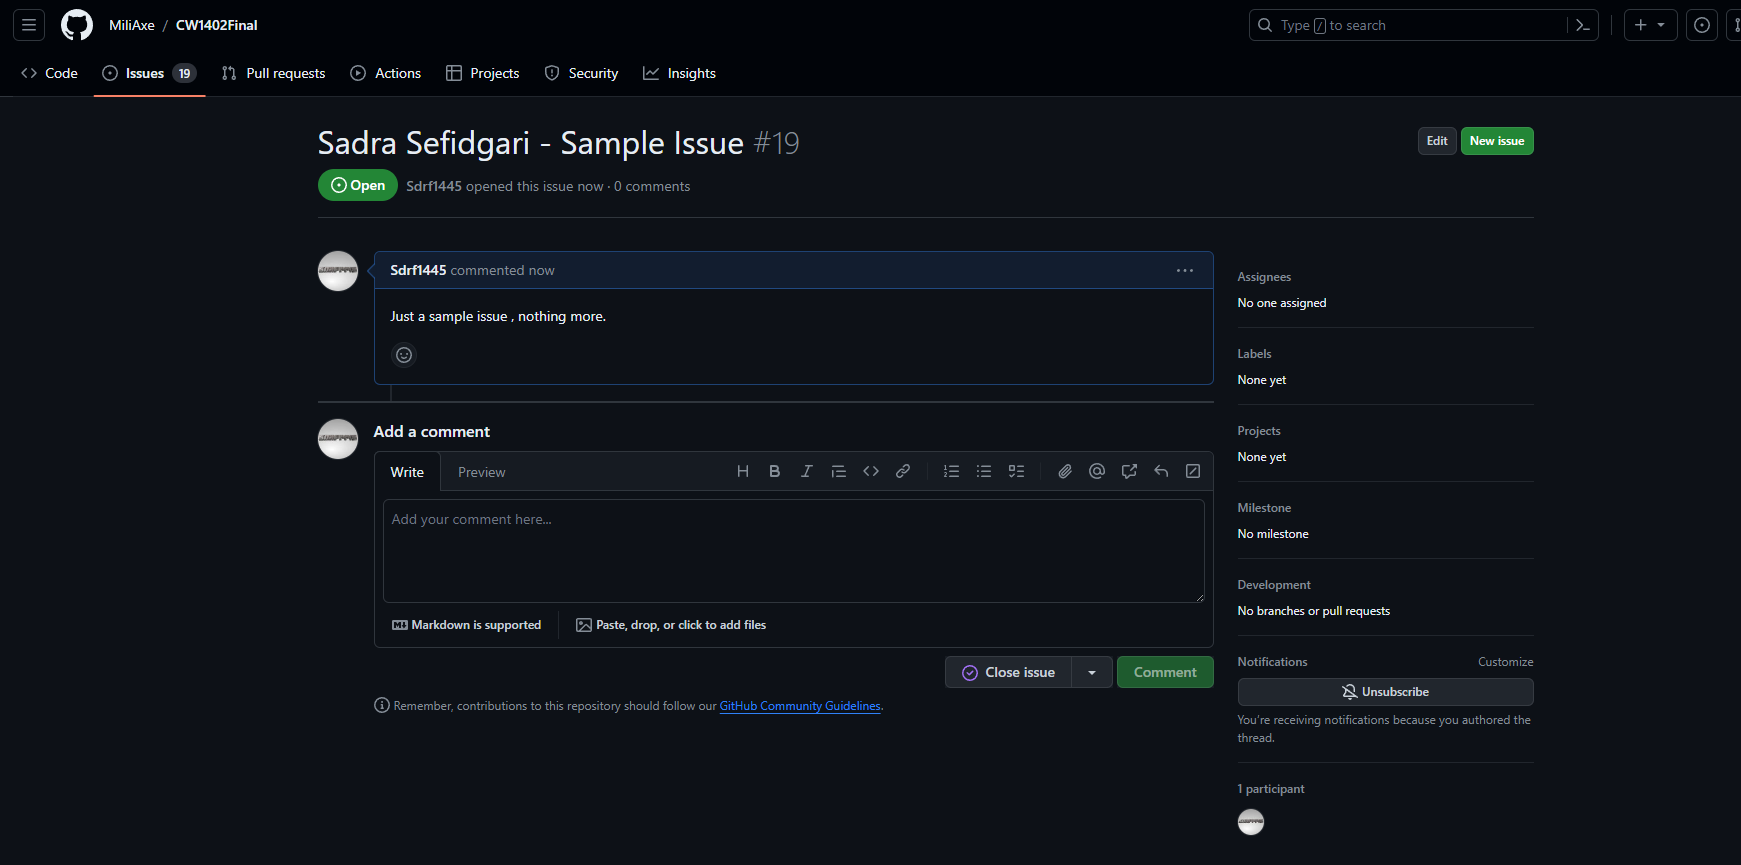
\includegraphics[width=0.8\textwidth]{screen.png}



   






  
\end{document}
